
\documentclass{abgabe}
\begin{document}

\begin{questions}
    \qformat{\thequestion. \textbf{\thequestiontitle} \hfill}
    \titledquestion{Klassendiagramm \& Objektdiagramm}

    Aus einer Protokoll-Notiz sind folgende Informationen festgehalten:
    Ein Reisender kann eine Einzelfahrkarte zu einem bestimmten Tarif (als Zeichenkette) und einem Preis (EUR) erwerben.
    Diese Fahrkarte legitimiert den Reisenden zur Nutzung einer bestimmten Strecke, die zwei Stationen miteinander verbindet.
    Die Strecke kennt dabei das Ausgangs- und Zielgleis.
    Die Station ist über den Stationsnamen eindeutig gekennzeichnet, der Reisende über seinen Namen.

    \begin{parts}
        \part
        Erstellen Sie ein fachliches Klassendiagramm.
        Identifitzieren Sie hierzu die Klassen, deren Beziehungen und die Attribute mit Datentypen.
        Modellieren Sie noch keine Methoden.
        Achten Sie auf die Multiplizitäten und Assoziationen.
        Alle Assoziationen sollen einen Namen und eine Leserichtung aufweisen.
        \begin{solution}
            \begin{center}
                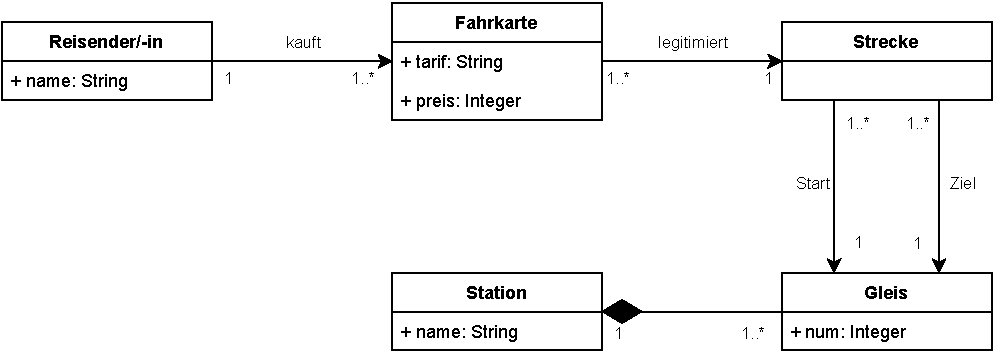
\includegraphics[width=\textwidth]{swt_h04_class.pdf}
            \end{center}
        \end{solution}

        \part
        Erstellen Sie auch ein passendes Objektdiagramm, das folgenden Sachverhalt beschreibt:

        Die Kundin Frau Müller fährt für 17.50€ mit dem Gute-Nacht-Tarif von Aachen Hbf (Gleis 7) nach Köln Hbf (Gleis 8)
        \begin{solution}
            \begin{center}
                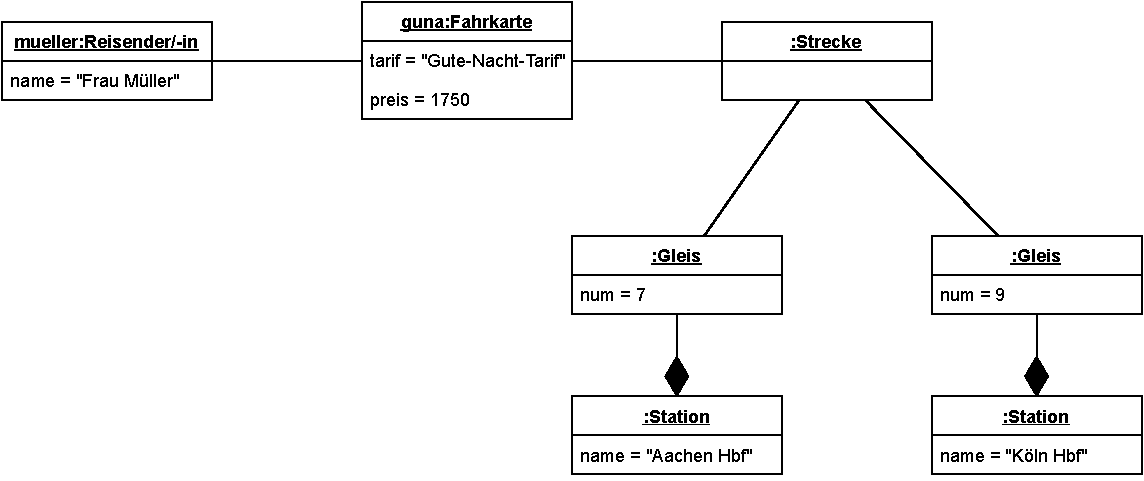
\includegraphics[width=\textwidth]{swt_h04_object.pdf}
            \end{center}
        \end{solution}
    \end{parts}

\end{questions}
\end{document}